% !TeX root = ../thesis.tex

\chapter{System}
\label{sec:system}

\section{Analoge Signalverarbeitung}
\label{sec:Signalverarbeitung}
Für die Übertragung von Signalen mithilfe einer LED müssen vorerst ein paar
grundlegende Überlegungen gemacht werden. Aus dem Kapitel Leuchtdiode sind
die grundsätzlichen Eigenschaften der LED, sowie ihre Kennlinie bekannt. Aus
diesen Erkenntnissen lässt sich direkt ausschließen, dass ein negativer Signalanteil
übertragen werden kann. Ebenso sollte man den stark nichtlinearen Teilbereich der
Kennlinie nicht nutzen, was dazu führt, dass die LED mit einem Offset betrieben
werden muss.Abbildung 6 zeigt die verschiedenen Stadien der Signalverarbeitung. Da es sich
hierbei um ein nichtlineares System handelt, können die Schritte nicht beliebig
vertauscht werden.Für die Schritte ”Offseterhöhung” und ”Amplitudenverstärkung” würde eine Schaltung
wie in Abbildung 7 gezeigt ausreichen. Hierbei wird der Offset über den Spannungsteiler
der DC-Quelle und dem Potentiometer P2 eingestellt. Die Verstärkung
der Amplitude erfolgt über die Verstärkung zwischen P1 und R3.




Treiber (https://wiki.analog.com/university/courses/electronics/text/chapter-4) ....

Die Spannungs-/Stromwandlung erfolgt mit der Schaltung aus Abbildung 9. Der
Operationsverstärker (OP) sorgt über eine Gegenkopplung seiner Ausgangsspannung immer dafür, dass zwischen seinen Eingängen kein Spannungsunterschied
herrscht. Bei anliegendem Signal am + Eingang versucht er daher diese Spannung
auszugleichen indem er eine Spannung am Ausgang erzeugt. Diese Spannung liegt
direkt am Gate des Metal Oxide Semiconductor Field Effect Transistors (MosFets)
an, welcher daraufhin durchschaltet und damit einen Stromfluß über die LED und
den Leistungswiderstand R2 erzeugt. Dieser Strom wiederum erzeugt über selbigen
Widerstand eine Anhebung des Potentials am - Eingang des OPs. Auf diese Weise
versucht der OP seine beiden Eingänge auf das gleiche Potential anzuheben. Da es
sich beim Leistungswiderstand R2 um einen sehr kleinen Widerstand handelt, wird
durch die LED, den MosFet und den Leistungswiderstand ein sehr hoher Strom
fließen welcher für eine hell leuchtende LED sorgt.

\begin{figure}[H]
	\centering
	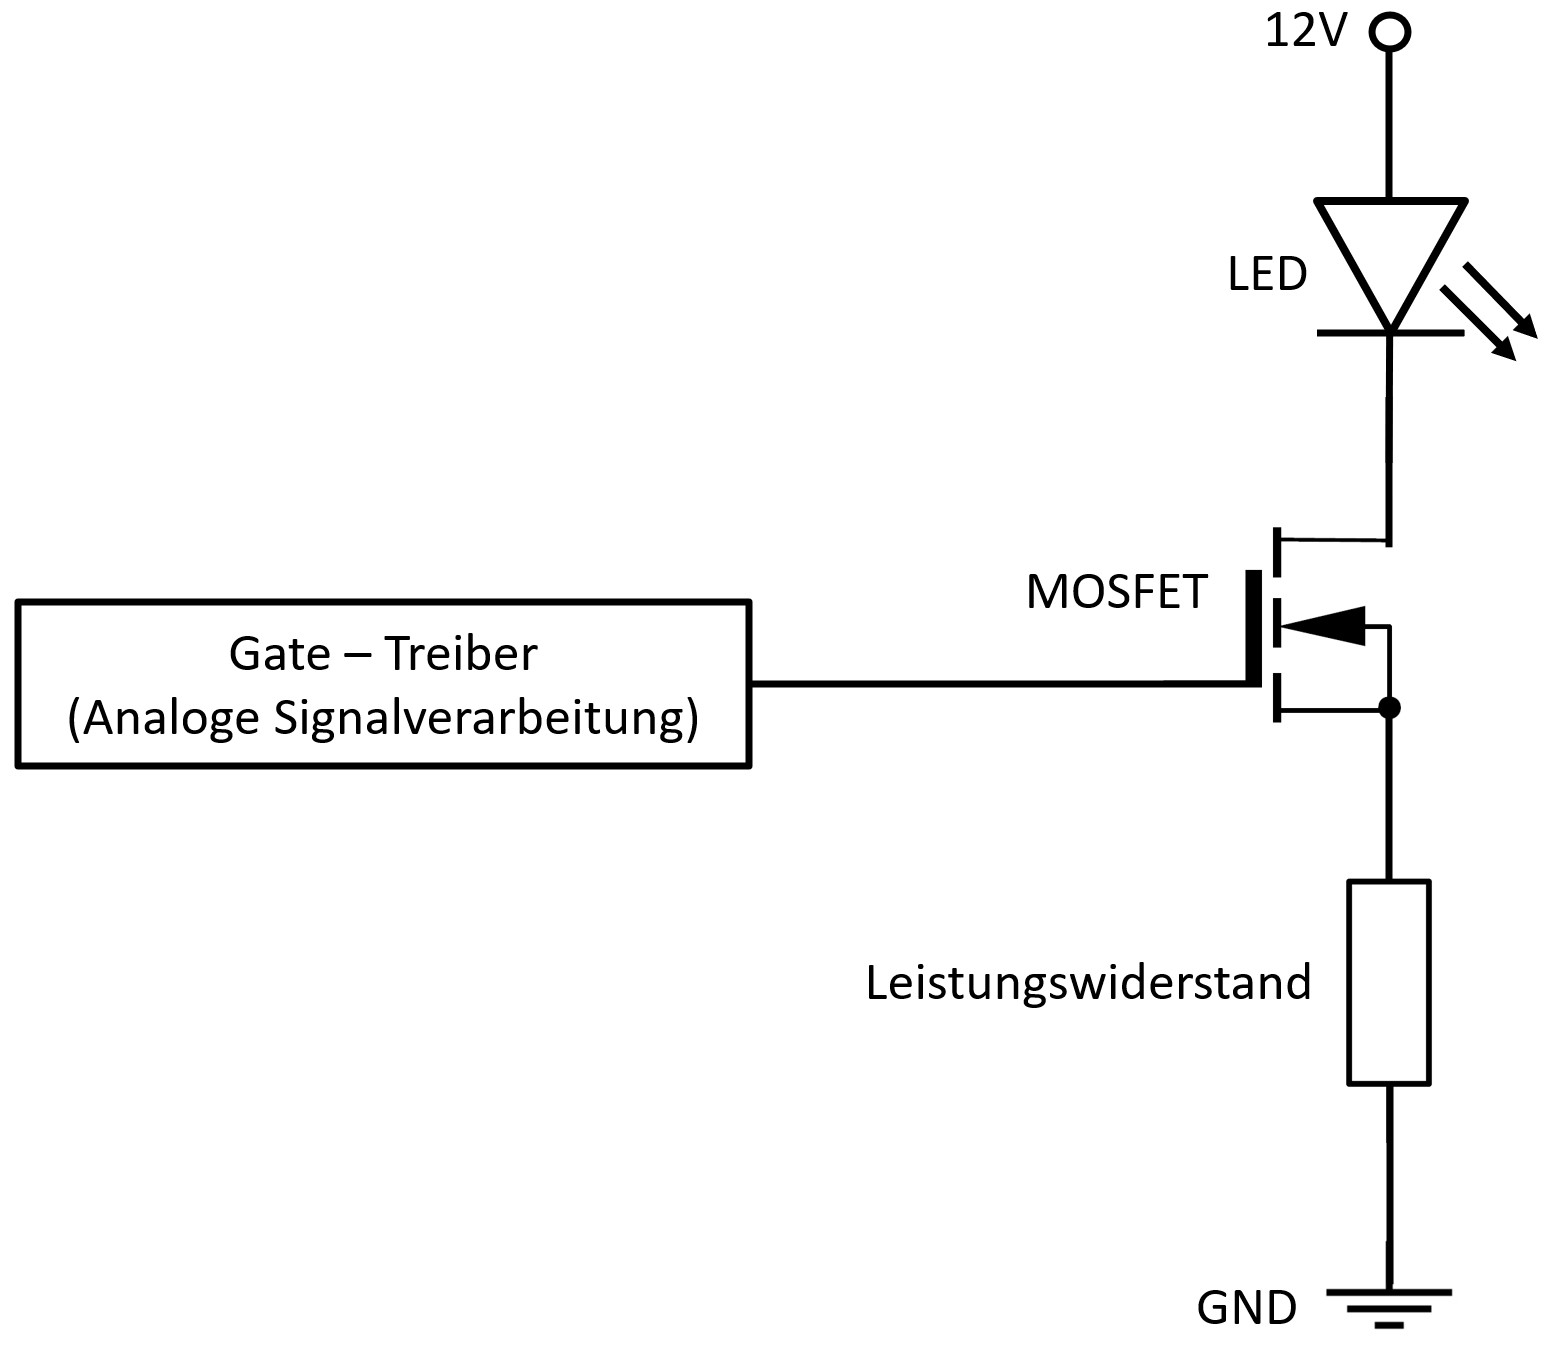
\includegraphics[width = 0.6 \textwidth ]{ledtreiber.jpg}
	\caption[Schaltung des LED- Treibers]{LED- Treiber} \gls{online:Eigen}
	\label{fig:ledtreiber}
\end{figure}

3.1.2 Probleme durch das Digitalpotentiometer
Wie aus dem Datenblatt des Digitalpotentiometers ersichtlich ist, kann dieses nur
mit Spannungen zwischen -0.6V absolut und +1V, ausgehend von der Versorgungsspannung
gemessen, arbeiten. Daher müssen die vorhandenen Signalverarbeitungsschritte
diesen Gegebenheiten angepasst werden.
Sieht man sich die Schaltung in Abbildung 8 an, fällt auf, dass der kritischste
Punkt für das Digitalpotentiometer der Einsatz in der Rückkopplung ist, da hier
auch niedrigere Spannungen als -0,6V am Ausgang des OPs auftreten können. Diese
Problematik soll Abbildung 10 verdeutlichen. Erhöht man die Amplitude des
Signals, würde man am Ausgang des OPs ein Signal bekommen, welches unter den
kritischen -0,6V liegt. Da das Digitalpotentiometer zwischen Ausgang und invertierendem
Eingang liegt, würde es nicht mehr richtig arbeiten.



\subsection{Simulation in LT-Spice}
\label{subsec:Unterabschnitt1}
 
\subsection{Platinenlayout in Eagle}
\label{subsec:Unterabschnitt12}

Beim Platinenlayout des Senders wurde besonders auf die Trennung von Signal und Leistungswege geachtet. Diese ist in Abbildung 14 mit einer Gelben Linie Mittig des Boards markiert.
Im unteren Bereich der Platine befinden sich Leistungswiderstand, LED, MosFet, Spannungswandler und der Operationsverstärker für die Stromquelle. Da in der Schaltung Ströme bis 1,41A fließen können und es somit zu EMV Störungen kommen kann, wurde der Signalweg in den oberen Bereich der Platine gelegt. Zudem
wurde die Leiterbahn zwischen Leuchtdiode, Transistor und Leistungswiderstand besonders breit ausgelegt, da hier große Ströme fließen. Auf der Platinen wurden für die Operationsverstärker und den Digitalpotentiometer
DIP Sockel verlötet. Das ermöglicht nachträglich einen einfachen Austausch der Bauelemente. Da die komplette Schaltung des Visible Light Senders auf die Größe einer kleinen Europlatine entworfen wurde, kam es zu Platzproblemen. Deshalb mussten zwei Leitungen auf der Rückseite der Platine verlegt werden. Diese sind in Abbildung 14 durch die beiden Blauen Linien dargestellt.
Um die Schaltung zusätzlich noch Störfester zu machen, wurden Freiflächen auf beiden Seiten der Platine mit Masse ausgefüllt. Des weiteren wurden noch zwei Pins an Masse, und ein Pin an 12V für Messungen und Fehlerüberprüfung angebracht. Der im oberen Teil des Boards eingezeichnete AUX Anschluss wurde nicht, wie in
Abbildung 14 gezeigt, an das Board gelötet, sondern am Deckel angebracht. Grund dafür ist das einfachere Anschließen des AUX Kabels. Um den Arduino stabil zu verbauen, wurde er an zwei Seiten befestigt.

\subsection{Thermisches Management}
\label{subsub:Unterunterabschnitt1}

Um die LED als Lichtquelle nutzen zu können, werden hohe Leistungen benötigt.
Im hellsten Betrieb der LED fließt ein Strom von 1,41A durch Transistor, LED
und Leistungswiderstand. Um der dadurch resultierenden Hitzeentwicklung entgegenzuwirken,
werden Transistor und Diode auf einem Kühlkörper montiert. Der
Leistungswiderstand liegt nahe am Transistorkühlkörper, darf aber nicht mit dem
Kühlkörper verbunden werden.
Ohne einen vorhandenen Kühlkörper würde sich der Transistor lt. Datenblatt um
62 $\circ$CC/W erhitzen. Da durch den geringen Leistungswiderstand und dem dadurch
resultierendem hohen Strom eine Leistung von ca. 5W in Hitze umgewandelt wird,
kann dies zur Zerstörung des Bauteils führen.
Zur Auslegung der Kühlkörper wurden folgende Berechnungen durchgeführt:

Hierbei ist:
–j die Maximale Sperrschichttemperatur in $\circ$C des Halbleiters (Herstellerangabe)
–A die Umgebungstemperatur in $\circ$CC
Pv die am zu kühlenden Halbleiter maximal anfallende Verlustleistung in
Watt
– RJC der Wärmewiderstand zwischen Sperrschicht und Gehäuse (Herstellerangabe)
– RCH der Wärmewiderstand zwischen Gehäuse und Kühlkörper
– RK der Wärmewiderstand des Kühlkörpers (Herstellerangabe)

\subsubsection{Kühlkörperberechnung des \gls{acr:MOSFET}s}
\label{subsub:Unterunterabschnitt1}

Für die Berechnung der Kühlkörper wurden Messungen zur Verlustleistung des
Transistors und der LED vorgenommen. Die maximalen Verluste werden bei voller
Helligkeit erzeugt.

– Leuchtdiode: 2,77V · 1,41A = 3,91W
– Transistor: 3,6V · 1,41A = 5,08W

Dadurch berechnet sich der Wärmewiderstand des Transistorkühlkörpers bei gewünschter
Chiptemperatur von 55$\circ$CC und einer Außentemperatur von 25$\circ$CC zu:
R = 55 $\circ$CC − 25$\circ$C5, 08W − (1.15$\circ$C/W + 0.3$\circ$C/W) = 4, 46$\circ$C/W
Ausgehend von der Gleichung 3 wurde ein Kühlkörper von 4,3 $\circ$CC/W gewählt.

\subsubsection{Kühlkörperberechnung der \gls{acr:LED}}
\label{subsub:Unterunterabschnitt1}

Bei der LED wurde eine geringere Chiptemperatur vorgesehen, da sie sich außen
an der Kante des Boards befindet und somit leicht berührbar ist. Zudem wurde
bei der Berechnung bewusst überdimensioniert. Dazu wird im folgenden mit einem
Wirkungsgrad der LED von 0 \%, und somit einer Verlustleistung von 100  \%
gerechnet, was dem Verhalten eines Widerstandes entspricht. LEDs haben jedoch
tatsächlich einen Wirkungsgrad von ca. 40 - 50 \%.
Der Kühlkörper für die LED berechnet sich wie folgt:

R = 40$\circ$ − 25$\circ$ 3, 91W − (1.25$\circ$C/W + 0.1$\circ$C/W) = 2, 49$\circ$C/W

Ausgehend von der Gleichung 4 wurde ein Kühlkörper von 2 C/W gewählt.

\subsection{Planung und Aufbau des Gehäuses}
\label{subsec:Unterabschnitt12}

Beim Entwurf des Gehäuses wurde so Platzsparend wie möglich gearbeitet, weshalb
der fest verbaute Arduino zwischen Leiterplatte und Deckel angebracht wurde.
Da sich Leistungswiderstand, Transistor und Leuchtdiode im Betrieb stark erhitzen,
wurden die zugehörigen Kühlkörper am Boden mithilfe von Abstandsbolzen
befestigt. Zusätzlich wurden im Deckel Freischnitte über den Kühlkörpern vorgenommen
um die nach oben steigende Luft möglichst gut abzuleiten. Für die
Versorgungsspannung der Schaltung gibt es zwei 4mm Anschlüsse, die oben am
Deckel angebracht wurden. Für die Datenübertragung wurde eine AUX Buchse im
Deckel verbaut.

\section{Software}
\label{sec:Software}
\subsection{Arduino Code zum Ansteuern der Digital Potentiometer}
\label{subsec:Unterabschnitt12}


\subsection{Übertragung mit Dream}
\label{subsec:dream}

Das Programm verfügt auf zwei verschiedene Möglichkeiten aufgerufen werden. Zum ersten im Sendemodus und zum zweiten im Empfangsmodus. Zudem bietet Dream umfangreiche Einstellungsoptionen um sowohl Rauschen oder aber auch andere Störungen zu minimieren. Die wichtigsten Parameter für die Korrekte Benutzung werden in dend
folgenden zwei Kapiteln näher erläutert.



\subsubsection{Dream Transmitter}
\label{subsubsec:dreamtx}
Zum Start der Software ”Dream” im Übertragungsmodus muss das Programm mit dem parameter ”- t” gestartet werden. Die einfachste Möglichkeit für einen Programmstart mit Parameter bietet eine Verknüpfung, welche wie in Abbildung 15 gezeigt, angepasst wird. Das Zielverzeichnis darf dabei nicht verändert werden! Dieser Schritt muss nur einmal gemacht werden und man kann jederzeit den Übertragungsmodus starten indem man die Dream software über diese geänderte Verknüpfung startet.

\begin{figure}[H]
	\centering
	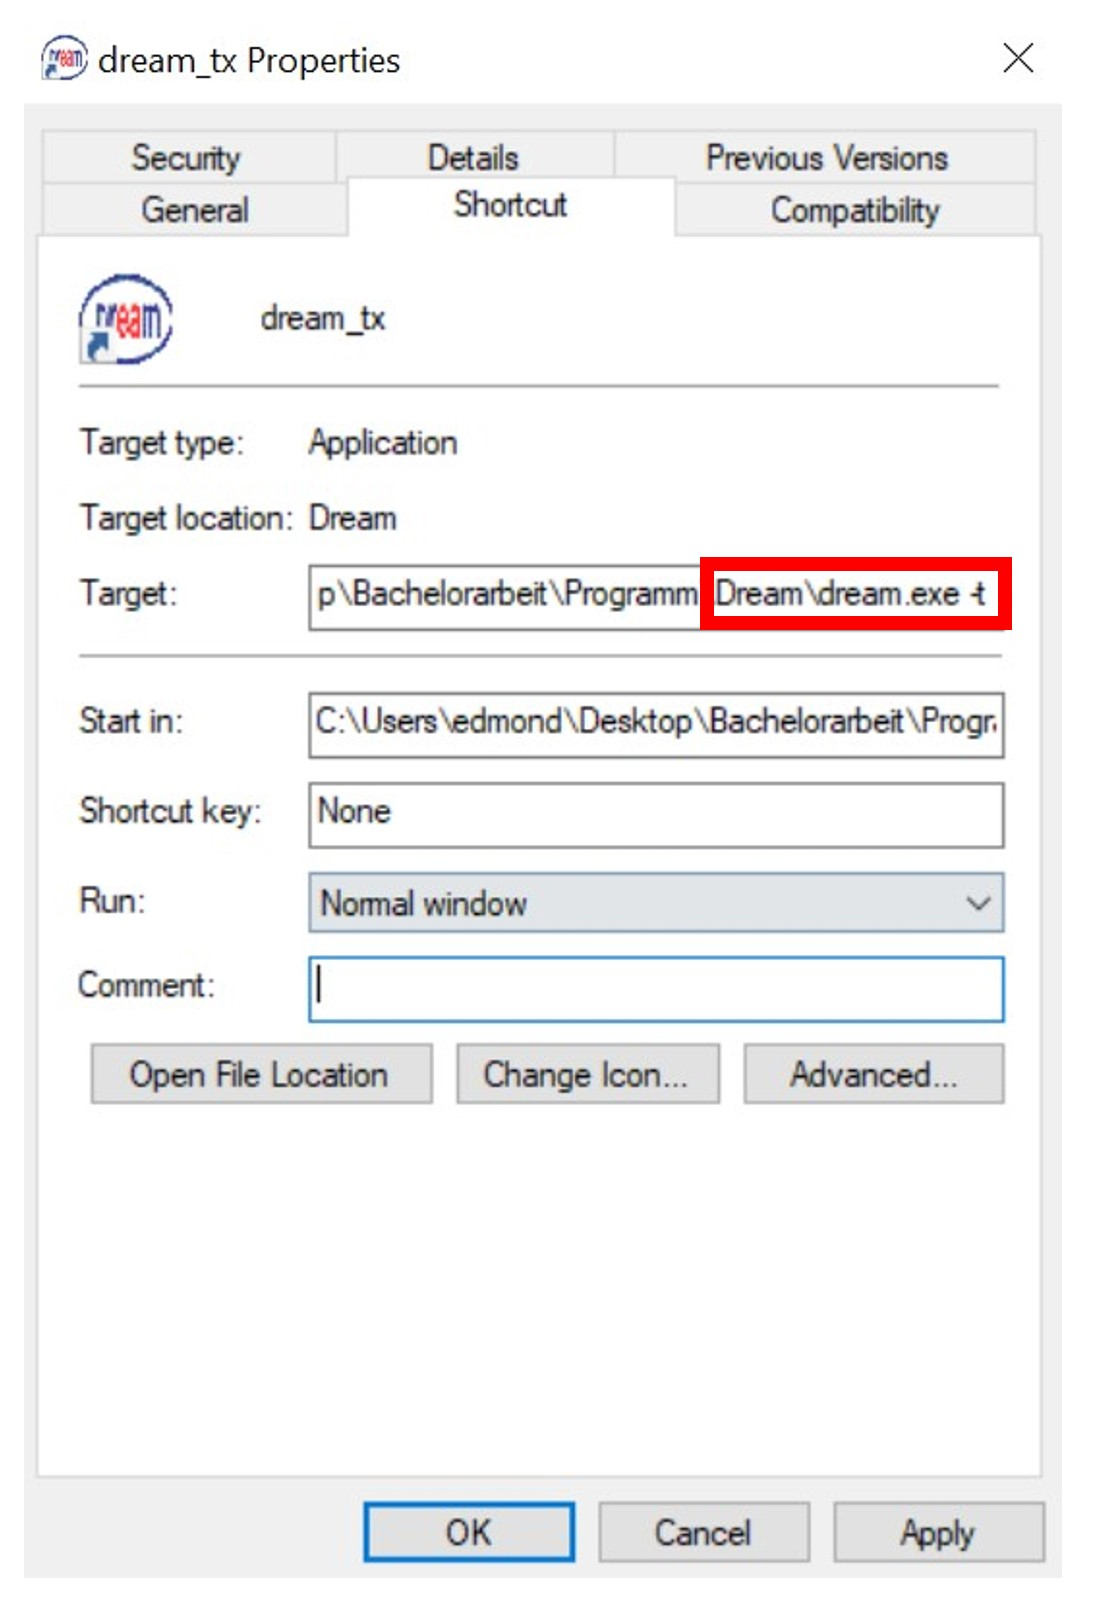
\includegraphics[width = 0.5 \textwidth ]{dreamtx.jpg}
	\caption[Modifizierung für den Sendemodus]{Modifizierung für den Sendemodus} \gls{online:Eigen}
	\label{fig:dreamtx}
\end{figure}

\begin{figure}[H]
	\centering
	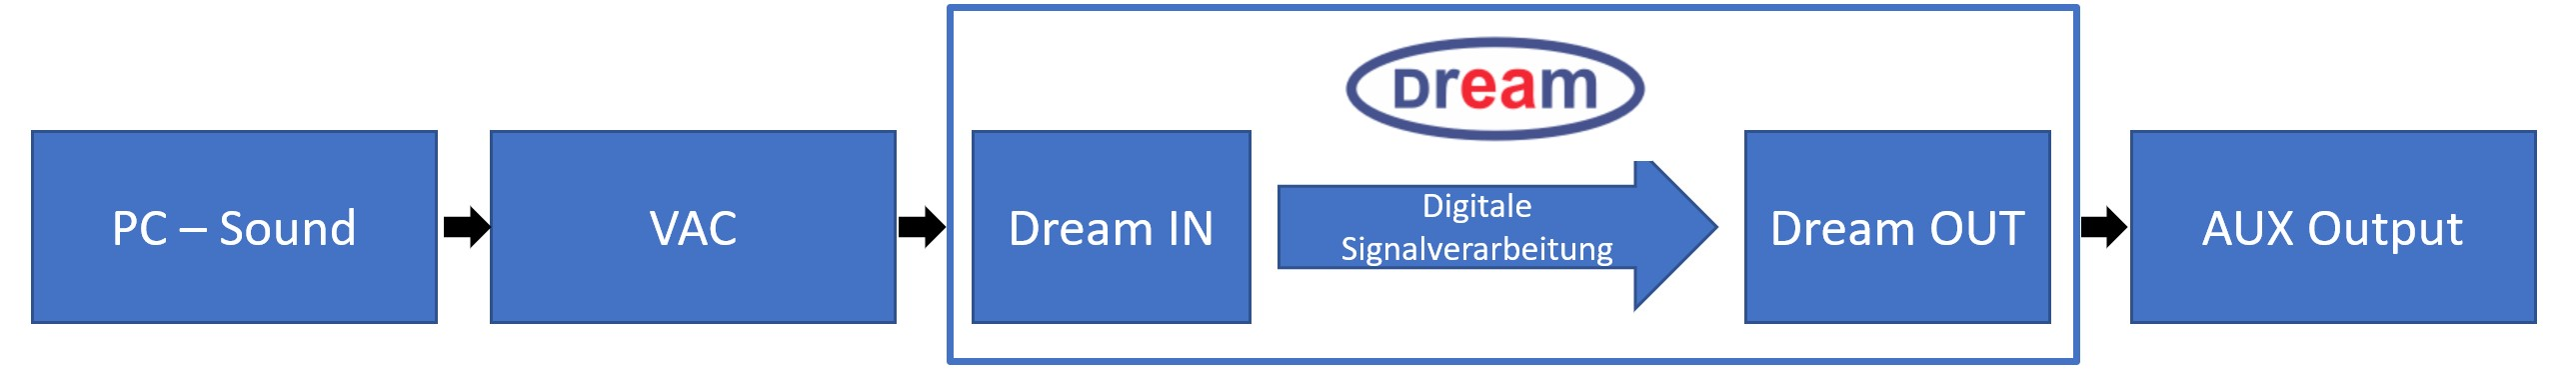
\includegraphics[width = 0.9 \textwidth ]{dreamtxeinstellung.jpg}
	\caption[Internes Audiorouting]{Internes Audiorouting} \gls{online:Eigen}
	\label{fig:dreamtxeinstellung}
\end{figure}

\subsubsection{Dream Receiver}
\label{subsec:Unterabschnitt12}

Der Evaluation Dialog liefert detaillierte Informationen über die empfangenen DRM-Parameter. Hier können Parameter sowie einige Diagramme eingesehen werden. In den folgenden Tabellen, werden für die Übertragung bedeutende Parameter näher erläutert.

\begin{table}[h]
	\begin{center}
		\begin{tabular}{p{0.3\linewidth} | p{0.7 \linewidth}}	
			\textbf{Measurements} & \\
			\hline
			\textbf{DC Frequency Offset} & Dieser Offset entspricht der resultierenden Soundkarten-Zwischenfrequenz des Frontends. Diese Frequenz ist nicht auf einen bestimmten Wert beschränkt, sondern nur darauf, dass das DRM-Spektrum vollständig innerhalb der Bandbreite der Soundkarte liegen muss.\\
			
			\textbf{Sample Frequency Offset} & Offset der Abtastrate des lokalen Computers zum DA-Wandler im Sender. \\
			
			\textbf{Doppler / Delay} & The Doppler frequency of the channel is estimated for the Wiener filter design of channel estimation in time direction. If linear interpolation is set for channel estimation in time direction, this estimation is not updated. The Doppler frequency is an indication of how fast the channel varies with time. The higher the frequency, the faster the channel changes are.
			The total delay time of the Power Delay Spectrum (PDS) is estimated from the impulse response estimation derived from the channel estimation. This delay corresponds to the range between the two vertical dashed black lines in the Impulse Response (IR) plot. \\
			\textbf{I/O Interface LED} & This LED shows the current status of the sound card interface. The yellow light shows that the audio output was corrected. Since the sample rate of the transmitter and local computer are different, from time to time the audio buffers will overflow or under run and a correction is necessary. When a correction occurs, a "click" sound can be heard. The red light shows that a buffer was lost in the sound card input stream. This can happen if a thread with a higher priority is at 100 and the Dream software cannot read the provided blocks fast enough. In this case the Dream software will instantly loose the synchronization and has to re-synchronize. Another reason for red light is that the processor is to slow for running the Dream software.
			\\
			\textbf{Time Sync Acq LED} & This LED shows the state of the timing acquisition (search for the beginning of an OFDM symbol). If the acquisition is done, this LED will stay green.
			\\
			\textbf{Frame Sync LED} & The DRM frame synchronization status is shown with this LED. This LED is also only active during acquisition state of the Dream receiver. In tracking mode this LED is always green.
			\\
			\textbf{FAC CRC LED} & This LED shows the Cyclic Redundancy Check (CRC) of the Fast Access Channel (FAC) of DRM. FAC is one of the three logical channels and is always modulated with a 4-QAM. If the FAC CRC check was successful, the receiver changes to tracking mode. The FAC LED is the indication whether the receiver is synchronized to a DRM transmission or not. \\
			\textbf{SRC CRC LED} & 	This LED shows the CRC check result of the Service Description Channel (SDC) which is one logical channel of the DRM stream. This data is transmitted in approx. 1 second intervals and contains information about station label, audio and data format etc. The error protection is normally lower than the protection of the FAC. Therefore this LED will turn to red earlier than the FAC LED in general. \\
			\textbf{MSC CRC LED} & This LED shows the status of the Main Service Channel (MSC). This channel contains the actual audio and data bits. The LED shows the CRC check of the AAC core decoder. The SBR has a separate CRC, but this status is not shown with this LED. If SBR CRC is wrong but the AAC CRC is ok one can still hear something (of course, the high frequencies are not there in this case). If this LED turns red, interruptions of the audio are heard. The yellow light shows that only one 40 ms audio frame CRC was wrong. This causes usually no hearable artifacts.\\
			
			
			
			
			
			\hline
		\end{tabular}
		\caption{Unterschrift  der Tabelle}
		\label{tab:Tabelle1}
	\end{center}
\end{table}

\begin{table}[h]
	\begin{center}
		\begin{tabular}{p{0.3\linewidth} | p{0.7\linewidth}}	
			
			\textbf{Parameters} &  \\
			\hline
			\textbf{DRM mode/ bandwidth} & In a DRM system, four possible robustness modes are defined to adapt the system to different channel conditions. According to the DRM standard:\newline
			\textbf{Mode A}: Gaussian channels, with minor fading\newline
			\textbf{Mode B}: Time and frequency selective channels, with longer delay spread\newline
			\textbf{Mode C}: As robustness mode B, but with higher Doppler spread\newline
			\textbf{Mode D}: As robustness mode B, but with severe delay and Doppler spread\newline
			The bandwidth is the gross bandwidth of the current DRM signal. \\
			\textbf{Interleaver Depth} & The symbol interleaver depth can be either short (approx. 400 ms) or long (approx. 2 s). The longer the interleaver the better the channel decoder can correct errors from slow fading signals. But the longer the interleaver length the longer the delay until audio can be heard (after a re-synchronization).
			\\
			\textbf{SDC / MSC Mode} & Shows the modulation type of the SDC and MSC channel. For the MSC channel, some hierarchical modes are defined which can provide a very strong protected service channel.
			\\
			\textbf{Prot. Level (B/A)} & The error protection level of the channel coder. For 64-QAM, there are four protection levels defined in the DRM standard. Protection level 0 has the highest protection whereas level 3 has the lowest protection. The letters A and B are the names of the higher and lower protected parts of a DRM block when Unequal Error Protection (UEP) is used. If Equal Error Protection (EEP) is used, only the protection level of part B is valid.
			\\
			\textbf{Number of Services} & This shows the number of audio and data services transmitted in the DRM stream. The maximum number of streams is four.
			\\
			\textbf{Received time - date} & This label shows the received time and date in UTC. This information is carried in the SDC channel.
			\\
			\hline
		\end{tabular}
		\caption{Unterschrift  der Tabelle}
		\label{tab:Tabelle1}
	\end{center}
\end{table}
\begin{table}[ht]
	\begin{center}
		\begin{tabular}{p{0.3\linewidth} | p{0.7\linewidth}}
			\textbf{Chart} & \\
			\hline
			\textbf{SNR} & Signal to Noise Ratio (SNR) estimation is plotted as a bar and as a value.
			\\
			\textbf{Main Plot} & Graphical display of different vectors of the DRM decoder. \\
			\hline
		\end{tabular}
		\caption{Unterschrift  der Tabelle}
		\label{tab:Tabelle1}
	\end{center}
\end{table}

\begin{table}[htb]
	\begin{center}
		\begin{tabular}{p{0.25\linewidth} | p{0.75\linewidth}}	
			
			\textbf{Advanced Settings} &  \\
			\hline
			\textbf{Frequency Interpolation} & With these settings the channel estimation method in frequency direction can be selected. The default value uses the most powerful algorithm.
			Wiener (default) - Wiener interpolation uses estimation of the statistics of the channel to design an optimal filter for noise reduction.
			Linear - Simple linear interpolation method to get the channel estimate. The real and imaginary parts of the estimated channel at the pilot positions are linearly interpolated. This algorithm causes the lowest CPU load but performs much worse than the Wiener interpolation at low SNR's.
			DFT Zero Pad: - Channel estimation method for the frequency direction using Discrete Fourier Transformation (DFT) to transform the channel estimation at the pilot positions to the time domain. A zero padding is applied to get a higher resolution in the frequency domain -> estimates at the data cells. This algorithm is very speed efficient but has problems at the edges of the OFDM spectrum due to the leakage effect. \\
			\textbf{Time Interpolation} & With these settings the channel estimation method in time direction can be selected. The default value uses the most powerful algorithm.
			Wiener (default) - Wiener interpolation uses estimation of the statistics of the channel to design an optimal filter for noise reduction.
			Linear - Simple linear interpolation method to get the channel estimate. The real and imaginary parts of the estimated channel at the pilot positions are interpolated linearly. This algorithm causes the lowest CPU load and the audio is decoded more quickly, but in general it performs worse than the Wiener interpolation especially at low SNR's. \\
			
			\textbf{Time Sync Tracking} & 	With these settings the time synchronization tracking methods can be selected.
			Guard Energy (default) - This algorithm utilizes the estimation of the impulse response and tries to maximize the energy in the guard-interval to set the correct timing.
			First Peak - This algorithm searches for the first peak in the estimated impulse response and moves this peak to the beginning of the guard-interval (timing tracking algorithm) \\
			
			\textbf{Flip Input Spectrum} & Checking this box will flip or invert the input spectrum. This is necessary if the mixer in the front-end uses the lower side band.
			\\
			
			\textbf{Mute Audio} & The audio can be muted by checking this box. The reaction of checking or unchecking this box is delayed by approx. 1 second due to the audio buffers.
			\\
			
			\textbf{MLC, Number of Iterations} & In DRM a multilevel channel coder is used. With this code it is possible to iterate the decoding process in the decoder to improve the decoding result. The more iterations are used the better the result will be. But switching to more iterations will increase the CPU load. Simulations showed that the first iteration (number of iterations = 1) gives the most improvement (approx. 1.5 dB at a BER of 10-4 on a Gaussian channel, Mode A, 10 kHz bandwidth). The improvement of the second iteration (number of iterations = 2) will be as small as 0.3 dB.
			The recommended number of iterations given in the DRM standard is one iteration (default value: number of iterations = 1).
			The selection is saved in the Dream.ini file. \\
			
			\textbf{Log File} & Checking this box causes Dream to write two kinds of log files about the current reception of an audio service using AAC source coding, a standard and a long log file. Both files are written to the directory were the Dream application is located.
			The standard log file DreamLog.txt is compatible to the log file created by the "DRM Software Radio". Each minute information about the average SNR, number of correct decoded FAC and number of correct decoded MSC blocks is recorded. The header of each log section also contains frequency, station label, bit-rate, mode and bandwidth. This file format is read by analyzer software like "DRMcalc" by Carsten Knütter.
			The long log file DreamLogLong.csv includes more detailed technical information: Frequency, date, time, average SNR, status of synchronization, status of FAC and MSC decoding, number of transmitted and decoded audio frames, Doppler frequency and the total delay time of the Power Delay Spectrum (PDS). It gets updated every second so that the resulting file size is growing quickly. The CSV file format can be handled by many spreadsheet applications like Microsoft Excel® or Sun StarOffice®.
			Known limitation: Due to a problem with QT timer implementation under Windows no Dream window should be moved or re-sized during logging! This problem does not exist in the Linux version of Dream.\\
			
			\textbf{Freq} & In the text field the current selected frequency on the front-end can be entered. This frequency will be written to the log file and saved in the Dream.ini file.
			\\
			
			\textbf{Save Audio as WAV} & Save the audio signal as stereo, 16-bit, 48 kHz sample rate PCM wave file. Checking this box will let the user choose a file name for the recording. \\
			
			\textbf{filter}& Checking the BP box will activate a band path filter to reduce interference from adjacent channels. The filter bandwidth is automatically set to the bandwidth of the current DRM signal.
			This filter should only be used in difficult reception situations because it increases CPU load noticeably.\\
			\hline
		\end{tabular}
		\caption{Unterschrift  der Tabelle}
		\label{tab:Tabelle1}
	\end{center}
\end{table}

